\icode{E-MD-CA-L3-261120-002}
如图所示，质量均为 \(m =\) \,\qty{3}{kg}的物块 \(A\)、\(B\) 紧挨着放置在粗糙的水平地面上，物块 \(A\) 的左侧连接一劲度系数为 \(k =\)\,\qty{100}{N/m} 的轻质弹簧，弹簧另一端固定在竖直墙壁上。开始时两物块压紧弹簧并恰好处于静止状态，现使物块 \(B\) 在水平外力 \(F\) 作用下向右做 \(a =\)\,\qty{2}{m/s^2} 的匀加速直线运动直至与 \(A\) 分离，已知两物块与地面的摩擦因数均为\(\mu = 0.5\)，\(g =\)\,\qty{10}{m/s^2}。求：
\begin{enumerate}
	\item 物块分离时，所加外力\(F\)的大小；
	\item \(A\)、\(B\)由静止到分离的时间。
\end{enumerate}

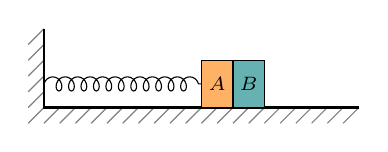
\begin{tikzpicture}[>=stealth,font=\scriptsize]
	\foreach \y in {-.2,0,.2,...,.8}
		\draw[gray] (-.2,\y)--++(.2,.2);
	\foreach \x in {0,.2,...,3.8}
		\draw[gray] (\x,-.2)--++(.2,.2);
	\draw[thick] (0,1)--(0,0)--(4,0);
	\draw[decoration={aspect=.8,segment length=4.5,amplitude=.9mm,coil},decorate] (0,.3)--(2,.3);
	\draw[fill=orange!60] (2,0) rectangle(2.4,.6)node[midway]{\(A\)};
	\draw[fill=teal!60] (2.4,0) rectangle(2.8,.6)node[midway]{\(B\)};
\end{tikzpicture}
\begin{answer}
	（1）\qty{21}{N}（2）\qty{0.3}{s}
\end{answer}